


% Header, overrides base

    % Make sure that the sphinx doc style knows who it inherits from.
    \def\sphinxdocclass{article}

    % Declare the document class
    \documentclass[letterpaper,10pt,english]{/usr/local/lib/python2.7/dist-packages/sphinx/texinputs/sphinxhowto}

    % Imports
    \usepackage[utf8]{inputenc}
    \DeclareUnicodeCharacter{00A0}{\\nobreakspace}
    \usepackage[T1]{fontenc}
    \usepackage{babel}
    \usepackage{times}
    \usepackage{import}
    \usepackage[Bjarne]{/usr/local/lib/python2.7/dist-packages/sphinx/texinputs/fncychap}
    \usepackage{longtable}
    \usepackage{/usr/local/lib/python2.7/dist-packages/sphinx/texinputs/sphinx}
    \usepackage{multirow}

    \usepackage{amsmath}
    \usepackage{amssymb}
    \usepackage{ucs}
    \usepackage{enumerate}

    % Used to make the Input/Output rules follow around the contents.
    \usepackage{needspace}

    % Pygments requirements
    \usepackage{fancyvrb}
    \usepackage{color}
    % ansi colors additions
    \definecolor{darkgreen}{rgb}{.12,.54,.11}
    \definecolor{lightgray}{gray}{.95}
    \definecolor{brown}{rgb}{0.54,0.27,0.07}
    \definecolor{purple}{rgb}{0.5,0.0,0.5}
    \definecolor{darkgray}{gray}{0.25}
    \definecolor{lightred}{rgb}{1.0,0.39,0.28}
    \definecolor{lightgreen}{rgb}{0.48,0.99,0.0}
    \definecolor{lightblue}{rgb}{0.53,0.81,0.92}
    \definecolor{lightpurple}{rgb}{0.87,0.63,0.87}
    \definecolor{lightcyan}{rgb}{0.5,1.0,0.83}

    % Needed to box output/input
    \usepackage{tikz}
        \usetikzlibrary{calc,arrows,shadows}
    \usepackage[framemethod=tikz]{mdframed}

    \usepackage{alltt}

    % Used to load and display graphics
    \usepackage{graphicx}
    \graphicspath{ {figs/} }
    \usepackage[Export]{adjustbox} % To resize

    % used so that images for notebooks which have spaces in the name can still be included
    \usepackage{grffile}


    % For formatting output while also word wrapping.
    \usepackage{listings}
    \lstset{breaklines=true}
    \lstset{basicstyle=\small\ttfamily}
    \def\smaller{\fontsize{9.5pt}{9.5pt}\selectfont}

    %Pygments definitions
    
\makeatletter
\def\PY@reset{\let\PY@it=\relax \let\PY@bf=\relax%
    \let\PY@ul=\relax \let\PY@tc=\relax%
    \let\PY@bc=\relax \let\PY@ff=\relax}
\def\PY@tok#1{\csname PY@tok@#1\endcsname}
\def\PY@toks#1+{\ifx\relax#1\empty\else%
    \PY@tok{#1}\expandafter\PY@toks\fi}
\def\PY@do#1{\PY@bc{\PY@tc{\PY@ul{%
    \PY@it{\PY@bf{\PY@ff{#1}}}}}}}
\def\PY#1#2{\PY@reset\PY@toks#1+\relax+\PY@do{#2}}

\expandafter\def\csname PY@tok@gd\endcsname{\def\PY@tc##1{\textcolor[rgb]{0.63,0.00,0.00}{##1}}}
\expandafter\def\csname PY@tok@gu\endcsname{\let\PY@bf=\textbf\def\PY@tc##1{\textcolor[rgb]{0.50,0.00,0.50}{##1}}}
\expandafter\def\csname PY@tok@gt\endcsname{\def\PY@tc##1{\textcolor[rgb]{0.00,0.27,0.87}{##1}}}
\expandafter\def\csname PY@tok@gs\endcsname{\let\PY@bf=\textbf}
\expandafter\def\csname PY@tok@gr\endcsname{\def\PY@tc##1{\textcolor[rgb]{1.00,0.00,0.00}{##1}}}
\expandafter\def\csname PY@tok@cm\endcsname{\let\PY@it=\textit\def\PY@tc##1{\textcolor[rgb]{0.25,0.50,0.50}{##1}}}
\expandafter\def\csname PY@tok@vg\endcsname{\def\PY@tc##1{\textcolor[rgb]{0.10,0.09,0.49}{##1}}}
\expandafter\def\csname PY@tok@m\endcsname{\def\PY@tc##1{\textcolor[rgb]{0.40,0.40,0.40}{##1}}}
\expandafter\def\csname PY@tok@mh\endcsname{\def\PY@tc##1{\textcolor[rgb]{0.40,0.40,0.40}{##1}}}
\expandafter\def\csname PY@tok@go\endcsname{\def\PY@tc##1{\textcolor[rgb]{0.53,0.53,0.53}{##1}}}
\expandafter\def\csname PY@tok@ge\endcsname{\let\PY@it=\textit}
\expandafter\def\csname PY@tok@vc\endcsname{\def\PY@tc##1{\textcolor[rgb]{0.10,0.09,0.49}{##1}}}
\expandafter\def\csname PY@tok@il\endcsname{\def\PY@tc##1{\textcolor[rgb]{0.40,0.40,0.40}{##1}}}
\expandafter\def\csname PY@tok@cs\endcsname{\let\PY@it=\textit\def\PY@tc##1{\textcolor[rgb]{0.25,0.50,0.50}{##1}}}
\expandafter\def\csname PY@tok@cp\endcsname{\def\PY@tc##1{\textcolor[rgb]{0.74,0.48,0.00}{##1}}}
\expandafter\def\csname PY@tok@gi\endcsname{\def\PY@tc##1{\textcolor[rgb]{0.00,0.63,0.00}{##1}}}
\expandafter\def\csname PY@tok@gh\endcsname{\let\PY@bf=\textbf\def\PY@tc##1{\textcolor[rgb]{0.00,0.00,0.50}{##1}}}
\expandafter\def\csname PY@tok@ni\endcsname{\let\PY@bf=\textbf\def\PY@tc##1{\textcolor[rgb]{0.60,0.60,0.60}{##1}}}
\expandafter\def\csname PY@tok@nl\endcsname{\def\PY@tc##1{\textcolor[rgb]{0.63,0.63,0.00}{##1}}}
\expandafter\def\csname PY@tok@nn\endcsname{\let\PY@bf=\textbf\def\PY@tc##1{\textcolor[rgb]{0.00,0.00,1.00}{##1}}}
\expandafter\def\csname PY@tok@no\endcsname{\def\PY@tc##1{\textcolor[rgb]{0.53,0.00,0.00}{##1}}}
\expandafter\def\csname PY@tok@na\endcsname{\def\PY@tc##1{\textcolor[rgb]{0.49,0.56,0.16}{##1}}}
\expandafter\def\csname PY@tok@nb\endcsname{\def\PY@tc##1{\textcolor[rgb]{0.00,0.50,0.00}{##1}}}
\expandafter\def\csname PY@tok@nc\endcsname{\let\PY@bf=\textbf\def\PY@tc##1{\textcolor[rgb]{0.00,0.00,1.00}{##1}}}
\expandafter\def\csname PY@tok@nd\endcsname{\def\PY@tc##1{\textcolor[rgb]{0.67,0.13,1.00}{##1}}}
\expandafter\def\csname PY@tok@ne\endcsname{\let\PY@bf=\textbf\def\PY@tc##1{\textcolor[rgb]{0.82,0.25,0.23}{##1}}}
\expandafter\def\csname PY@tok@nf\endcsname{\def\PY@tc##1{\textcolor[rgb]{0.00,0.00,1.00}{##1}}}
\expandafter\def\csname PY@tok@si\endcsname{\let\PY@bf=\textbf\def\PY@tc##1{\textcolor[rgb]{0.73,0.40,0.53}{##1}}}
\expandafter\def\csname PY@tok@s2\endcsname{\def\PY@tc##1{\textcolor[rgb]{0.73,0.13,0.13}{##1}}}
\expandafter\def\csname PY@tok@vi\endcsname{\def\PY@tc##1{\textcolor[rgb]{0.10,0.09,0.49}{##1}}}
\expandafter\def\csname PY@tok@nt\endcsname{\let\PY@bf=\textbf\def\PY@tc##1{\textcolor[rgb]{0.00,0.50,0.00}{##1}}}
\expandafter\def\csname PY@tok@nv\endcsname{\def\PY@tc##1{\textcolor[rgb]{0.10,0.09,0.49}{##1}}}
\expandafter\def\csname PY@tok@s1\endcsname{\def\PY@tc##1{\textcolor[rgb]{0.73,0.13,0.13}{##1}}}
\expandafter\def\csname PY@tok@sh\endcsname{\def\PY@tc##1{\textcolor[rgb]{0.73,0.13,0.13}{##1}}}
\expandafter\def\csname PY@tok@sc\endcsname{\def\PY@tc##1{\textcolor[rgb]{0.73,0.13,0.13}{##1}}}
\expandafter\def\csname PY@tok@sx\endcsname{\def\PY@tc##1{\textcolor[rgb]{0.00,0.50,0.00}{##1}}}
\expandafter\def\csname PY@tok@bp\endcsname{\def\PY@tc##1{\textcolor[rgb]{0.00,0.50,0.00}{##1}}}
\expandafter\def\csname PY@tok@c1\endcsname{\let\PY@it=\textit\def\PY@tc##1{\textcolor[rgb]{0.25,0.50,0.50}{##1}}}
\expandafter\def\csname PY@tok@kc\endcsname{\let\PY@bf=\textbf\def\PY@tc##1{\textcolor[rgb]{0.00,0.50,0.00}{##1}}}
\expandafter\def\csname PY@tok@c\endcsname{\let\PY@it=\textit\def\PY@tc##1{\textcolor[rgb]{0.25,0.50,0.50}{##1}}}
\expandafter\def\csname PY@tok@mf\endcsname{\def\PY@tc##1{\textcolor[rgb]{0.40,0.40,0.40}{##1}}}
\expandafter\def\csname PY@tok@err\endcsname{\def\PY@bc##1{\setlength{\fboxsep}{0pt}\fcolorbox[rgb]{1.00,0.00,0.00}{1,1,1}{\strut ##1}}}
\expandafter\def\csname PY@tok@kd\endcsname{\let\PY@bf=\textbf\def\PY@tc##1{\textcolor[rgb]{0.00,0.50,0.00}{##1}}}
\expandafter\def\csname PY@tok@ss\endcsname{\def\PY@tc##1{\textcolor[rgb]{0.10,0.09,0.49}{##1}}}
\expandafter\def\csname PY@tok@sr\endcsname{\def\PY@tc##1{\textcolor[rgb]{0.73,0.40,0.53}{##1}}}
\expandafter\def\csname PY@tok@mo\endcsname{\def\PY@tc##1{\textcolor[rgb]{0.40,0.40,0.40}{##1}}}
\expandafter\def\csname PY@tok@kn\endcsname{\let\PY@bf=\textbf\def\PY@tc##1{\textcolor[rgb]{0.00,0.50,0.00}{##1}}}
\expandafter\def\csname PY@tok@mi\endcsname{\def\PY@tc##1{\textcolor[rgb]{0.40,0.40,0.40}{##1}}}
\expandafter\def\csname PY@tok@gp\endcsname{\let\PY@bf=\textbf\def\PY@tc##1{\textcolor[rgb]{0.00,0.00,0.50}{##1}}}
\expandafter\def\csname PY@tok@o\endcsname{\def\PY@tc##1{\textcolor[rgb]{0.40,0.40,0.40}{##1}}}
\expandafter\def\csname PY@tok@kr\endcsname{\let\PY@bf=\textbf\def\PY@tc##1{\textcolor[rgb]{0.00,0.50,0.00}{##1}}}
\expandafter\def\csname PY@tok@s\endcsname{\def\PY@tc##1{\textcolor[rgb]{0.73,0.13,0.13}{##1}}}
\expandafter\def\csname PY@tok@kp\endcsname{\def\PY@tc##1{\textcolor[rgb]{0.00,0.50,0.00}{##1}}}
\expandafter\def\csname PY@tok@w\endcsname{\def\PY@tc##1{\textcolor[rgb]{0.73,0.73,0.73}{##1}}}
\expandafter\def\csname PY@tok@kt\endcsname{\def\PY@tc##1{\textcolor[rgb]{0.69,0.00,0.25}{##1}}}
\expandafter\def\csname PY@tok@ow\endcsname{\let\PY@bf=\textbf\def\PY@tc##1{\textcolor[rgb]{0.67,0.13,1.00}{##1}}}
\expandafter\def\csname PY@tok@sb\endcsname{\def\PY@tc##1{\textcolor[rgb]{0.73,0.13,0.13}{##1}}}
\expandafter\def\csname PY@tok@k\endcsname{\let\PY@bf=\textbf\def\PY@tc##1{\textcolor[rgb]{0.00,0.50,0.00}{##1}}}
\expandafter\def\csname PY@tok@se\endcsname{\let\PY@bf=\textbf\def\PY@tc##1{\textcolor[rgb]{0.73,0.40,0.13}{##1}}}
\expandafter\def\csname PY@tok@sd\endcsname{\let\PY@it=\textit\def\PY@tc##1{\textcolor[rgb]{0.73,0.13,0.13}{##1}}}

\def\PYZbs{\char`\\}
\def\PYZus{\char`\_}
\def\PYZob{\char`\{}
\def\PYZcb{\char`\}}
\def\PYZca{\char`\^}
\def\PYZam{\char`\&}
\def\PYZlt{\char`\<}
\def\PYZgt{\char`\>}
\def\PYZsh{\char`\#}
\def\PYZpc{\char`\%}
\def\PYZdl{\char`\$}
\def\PYZhy{\char`\-}
\def\PYZsq{\char`\'}
\def\PYZdq{\char`\"}
\def\PYZti{\char`\~}
% for compatibility with earlier versions
\def\PYZat{@}
\def\PYZlb{[}
\def\PYZrb{]}
\makeatother


    %Set pygments styles if needed...
    
        \definecolor{nbframe-border}{rgb}{0.867,0.867,0.867}
        \definecolor{nbframe-bg}{rgb}{0.969,0.969,0.969}
        \definecolor{nbframe-in-prompt}{rgb}{0.0,0.0,0.502}
        \definecolor{nbframe-out-prompt}{rgb}{0.545,0.0,0.0}

        \newenvironment{ColorVerbatim}
        {\begin{mdframed}[%
            roundcorner=1.0pt, %
            backgroundcolor=nbframe-bg, %
            userdefinedwidth=1\linewidth, %
            leftmargin=0.1\linewidth, %
            innerleftmargin=0pt, %
            innerrightmargin=0pt, %
            linecolor=nbframe-border, %
            linewidth=1pt, %
            usetwoside=false, %
            everyline=true, %
            innerlinewidth=3pt, %
            innerlinecolor=nbframe-bg, %
            middlelinewidth=1pt, %
            middlelinecolor=nbframe-bg, %
            outerlinewidth=0.5pt, %
            outerlinecolor=nbframe-border, %
            needspace=0pt
        ]}
        {\end{mdframed}}
        
        \newenvironment{InvisibleVerbatim}
        {\begin{mdframed}[leftmargin=0.1\linewidth,innerleftmargin=3pt,innerrightmargin=3pt, userdefinedwidth=1\linewidth, linewidth=0pt, linecolor=white, usetwoside=false]}
        {\end{mdframed}}

        \renewenvironment{Verbatim}[1][\unskip]
        {\begin{alltt}\smaller}
        {\end{alltt}}
    

    % Help prevent overflowing lines due to urls and other hard-to-break 
    % entities.  This doesn't catch everything...
    \sloppy

    % Document level variables
    \title{Trabalho 1}
    \date{March 5, 2014}
    \release{}
    \author{Unknown Author}
    \renewcommand{\releasename}{}

    % TODO: Add option for the user to specify a logo for his/her export.
    \newcommand{\sphinxlogo}{}

    % Make the index page of the document.
    \makeindex

    % Import sphinx document type specifics.
     


% Body

    % Start of the document
    \begin{document}

        
            \maketitle
        

        


        
        

    % Make sure that atleast 4 lines are below the HR
    \needspace{4\baselineskip}

    
        \vspace{6pt}
        \makebox[0.1\linewidth]{\smaller\hfill\tt\color{nbframe-in-prompt}In\hspace{4pt}{[}174{]}:\hspace{4pt}}\\*
        \vspace{-2.65\baselineskip}
        \begin{ColorVerbatim}
            \vspace{-0.7\baselineskip}
            \begin{Verbatim}[commandchars=\\\{\}]
\PY{k+kn}{import} \PY{n+nn}{warnings}
\PY{n}{warnings}\PY{o}{.}\PY{n}{filterwarnings}\PY{p}{(}\PY{l+s}{\PYZsq{}}\PY{l+s}{ignore}\PY{l+s}{\PYZsq{}}\PY{p}{)}
\end{Verbatim}

            
                \vspace{-0.2\baselineskip}
            
        \end{ColorVerbatim}
    
\part{Função para carregamento de dados}
Função que carrega os dados dos arquivos, retornando dois arrays, um
contendo as n-1 primeiras colunas e outro com a n-ésima coluna.


    % Make sure that atleast 4 lines are below the HR
    \needspace{4\baselineskip}

    
        \vspace{6pt}
        \makebox[0.1\linewidth]{\smaller\hfill\tt\color{nbframe-in-prompt}In\hspace{4pt}{[}175{]}:\hspace{4pt}}\\*
        \vspace{-2.65\baselineskip}
        \begin{ColorVerbatim}
            \vspace{-0.7\baselineskip}
            \begin{Verbatim}[commandchars=\\\{\}]
\PY{n}{PATH\PYZus{}DADOS} \PY{o}{=} \PY{l+s}{\PYZdq{}}\PY{l+s}{Dados Exercicio 1}\PY{l+s}{\PYZdq{}}
\PY{n}{FILENAMES} \PY{o}{=} \PY{p}{[}\PY{l+s}{\PYZdq{}}\PY{l+s}{ex1data1.txt}\PY{l+s}{\PYZdq{}}\PY{p}{,} \PY{l+s}{\PYZdq{}}\PY{l+s}{ex1data2.txt}\PY{l+s}{\PYZdq{}}\PY{p}{,} \PY{l+s}{\PYZdq{}}\PY{l+s}{ex1data3.txt}\PY{l+s}{\PYZdq{}}\PY{p}{]}

\PY{c}{\PYZsh{} lê de um arquivo de dados com linhas de samples}
\PY{c}{\PYZsh{} retorna um array de features e um de ys, sendo o primeiro formado pelos n\PYZhy{}1 primeiros números }
\PY{c}{\PYZsh{}     e o último formado pelos últimos números}
\PY{k}{def} \PY{n+nf}{carregar}\PY{p}{(}\PY{n}{filename}\PY{p}{,} \PY{n}{delimiter}\PY{o}{=}\PY{l+s}{\PYZdq{}}\PY{l+s}{ }\PY{l+s}{\PYZdq{}}\PY{p}{)}\PY{p}{:}
    \PY{k+kn}{import} \PY{n+nn}{csv}
    \PY{k+kn}{import} \PY{n+nn}{os}
    
    \PY{n}{reader} \PY{o}{=} \PY{n}{csv}\PY{o}{.}\PY{n}{reader}\PY{p}{(}\PY{n+nb}{open}\PY{p}{(}\PY{n}{os}\PY{o}{.}\PY{n}{path}\PY{o}{.}\PY{n}{join}\PY{p}{(}\PY{n}{PATH\PYZus{}DADOS}\PY{p}{,} \PY{n}{filename}\PY{p}{)}\PY{p}{)}\PY{p}{,} \PY{n}{delimiter}\PY{o}{=}\PY{n}{delimiter}\PY{p}{)}
    
    \PY{n}{values\PYZus{}X} \PY{o}{=} \PY{p}{[}\PY{p}{]}
    \PY{n}{values\PYZus{}Y} \PY{o}{=} \PY{p}{[}\PY{p}{]}

    \PY{k}{for} \PY{n}{row} \PY{o+ow}{in} \PY{n}{reader}\PY{p}{:}
        \PY{n}{values\PYZus{}X}\PY{o}{.}\PY{n}{append}\PY{p}{(}\PY{p}{[}\PY{n+nb}{float}\PY{p}{(}\PY{n}{x}\PY{p}{)} \PY{k}{for} \PY{n}{x} \PY{o+ow}{in} \PY{n}{row}\PY{p}{[}\PY{p}{:}\PY{o}{\PYZhy{}}\PY{l+m+mi}{1}\PY{p}{]}\PY{p}{]}\PY{p}{)}
        \PY{n}{values\PYZus{}Y}\PY{o}{.}\PY{n}{append}\PY{p}{(}\PY{n+nb}{float}\PY{p}{(}\PY{n}{row}\PY{p}{[}\PY{o}{\PYZhy{}}\PY{l+m+mi}{1}\PY{p}{]}\PY{p}{)}\PY{p}{)}
    
    \PY{k+kn}{import} \PY{n+nn}{numpy} \PY{k+kn}{as} \PY{n+nn}{np}

    \PY{k}{return} \PY{n}{np}\PY{o}{.}\PY{n}{array}\PY{p}{(}\PY{n}{values\PYZus{}X}\PY{p}{)}\PY{p}{,} \PY{n}{np}\PY{o}{.}\PY{n}{array}\PY{p}{(}\PY{n}{values\PYZus{}Y}\PY{p}{)}
\end{Verbatim}

            
                \vspace{-0.2\baselineskip}
            
        \end{ColorVerbatim}
    
\part{Função para plotar o gráfico com duas dimensões}

    % Make sure that atleast 4 lines are below the HR
    \needspace{4\baselineskip}

    
        \vspace{6pt}
        \makebox[0.1\linewidth]{\smaller\hfill\tt\color{nbframe-in-prompt}In\hspace{4pt}{[}176{]}:\hspace{4pt}}\\*
        \vspace{-2.65\baselineskip}
        \begin{ColorVerbatim}
            \vspace{-0.7\baselineskip}
            \begin{Verbatim}[commandchars=\\\{\}]
\PY{k}{def} \PY{n+nf}{plot2d}\PY{p}{(}\PY{n}{X}\PY{p}{,} \PY{n}{Y}\PY{p}{,} \PY{n}{color}\PY{o}{=}\PY{n+nb+bp}{None}\PY{p}{)}\PY{p}{:}
    \PY{k+kn}{from} \PY{n+nn}{matplotlib} \PY{k+kn}{import} \PY{n}{pyplot} \PY{k}{as} \PY{n}{pl}
        
    \PY{n}{line} \PY{o}{=} \PY{n}{pl}\PY{o}{.}\PY{n}{plot}\PY{p}{(}\PY{n}{X}\PY{p}{,} \PY{n}{Y}\PY{p}{)}
    \PY{k}{if} \PY{o+ow}{not} \PY{n}{color} \PY{o+ow}{is} \PY{n+nb+bp}{None}\PY{p}{:}
        \PY{n}{pyplot}\PY{o}{.}\PY{n}{setp}\PY{p}{(}\PY{n}{line}\PY{p}{,} \PY{n}{color}\PY{o}{=}\PY{n}{color}\PY{p}{)}

\PY{k}{def} \PY{n+nf}{scatter2d}\PY{p}{(}\PY{n}{X}\PY{p}{,} \PY{n}{Y}\PY{p}{)}\PY{p}{:}
    \PY{k+kn}{from} \PY{n+nn}{matplotlib} \PY{k+kn}{import} \PY{n}{pyplot} \PY{k}{as} \PY{n}{pl}
    
    \PY{n}{pl}\PY{o}{.}\PY{n}{scatter}\PY{p}{(}\PY{n}{X}\PY{p}{,} \PY{n}{Y}\PY{p}{)}
\end{Verbatim}

            
                \vspace{-0.2\baselineskip}
            
        \end{ColorVerbatim}
    
\part{Questão 1}\subsubsection{Figura com os dados}

    % Make sure that atleast 4 lines are below the HR
    \needspace{4\baselineskip}

    
        \vspace{6pt}
        \makebox[0.1\linewidth]{\smaller\hfill\tt\color{nbframe-in-prompt}In\hspace{4pt}{[}177{]}:\hspace{4pt}}\\*
        \vspace{-2.65\baselineskip}
        \begin{ColorVerbatim}
            \vspace{-0.7\baselineskip}
            \begin{Verbatim}[commandchars=\\\{\}]
\PY{n}{X}\PY{p}{,} \PY{n}{Y} \PY{o}{=} \PY{n}{carregar}\PY{p}{(}\PY{n}{FILENAMES}\PY{p}{[}\PY{l+m+mi}{0}\PY{p}{]}\PY{p}{)}
\PY{n}{scatter2d}\PY{p}{(}\PY{n}{X}\PY{p}{,} \PY{n}{Y}\PY{p}{)}
\end{Verbatim}

            
                \vspace{-0.2\baselineskip}
            
        \end{ColorVerbatim}
    

    

        % If the first block is an image, minipage the image.  Else
        % request a certain amount of space for the input text.
        \needspace{4\baselineskip}
        
        

            % Add document contents.
            
                \begin{InvisibleVerbatim}
                \vspace{-0.5\baselineskip}
    \begin{center}
    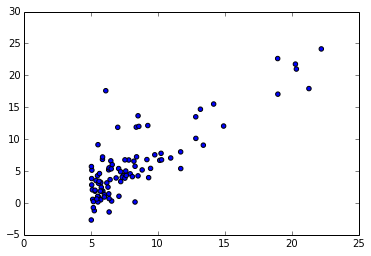
\includegraphics[max size={\textwidth}{\textheight}]{Trabalho 1_files/Trabalho 1_8_0.png}
    \par
    \end{center}
    
            \end{InvisibleVerbatim}
            
        
    
\subsubsection{Comentários: Um modelo de regressão linear parece ser adequado para os
dados em questão? Comente.}
Essa questão só pode ser respondida a partir da definição de
"adequado". Ela envolve aspectos como a precisão que se deseja
alcançar com o modelo e quão próximo dos dados de treinamento espera-
se que os dados a serem predizidos sejam.
Pelo gráfico, os dados não parecem possuir uma boa aproximação por uma
reta, por possuir, para valores próximos de x, variações não
monotônicas de y.
\subsubsection{\begin{itemize}
\itemsep1pt\parskip0pt\parsep0pt
\item
  Implemente o algoritmo do gradiente descendente estocástico para
  encontrar os coeficientes da regressão.
\end{itemize}}

    % Make sure that atleast 4 lines are below the HR
    \needspace{4\baselineskip}

    
        \vspace{6pt}
        \makebox[0.1\linewidth]{\smaller\hfill\tt\color{nbframe-in-prompt}In\hspace{4pt}{[}178{]}:\hspace{4pt}}\\*
        \vspace{-2.65\baselineskip}
        \begin{ColorVerbatim}
            \vspace{-0.7\baselineskip}
            \begin{Verbatim}[commandchars=\\\{\}]
\PY{c}{\PYZsh{} retorna o EQM}
\PY{k}{def} \PY{n+nf}{eqm}\PY{p}{(}\PY{n}{gerado}\PY{p}{,} \PY{n}{esperado}\PY{p}{)}\PY{p}{:}
    \PY{n}{resultado} \PY{o}{=} \PY{l+m+mf}{0.}
    
    \PY{k}{for} \PY{n}{g}\PY{p}{,} \PY{n}{e} \PY{o+ow}{in} \PY{n+nb}{zip}\PY{p}{(}\PY{n}{gerado}\PY{p}{,} \PY{n}{esperado}\PY{p}{)}\PY{p}{:}
        \PY{n}{erro} \PY{o}{=} \PY{n}{g} \PY{o}{\PYZhy{}} \PY{n}{e}
        \PY{n}{erro\PYZus{}quadrado} \PY{o}{=} \PY{n}{erro}\PY{o}{*}\PY{o}{*}\PY{l+m+mi}{2}
        
        \PY{n}{resultado} \PY{o}{+}\PY{o}{=} \PY{n}{erro\PYZus{}quadrado}
        
    \PY{n}{resultado} \PY{o}{/}\PY{o}{=} \PY{n+nb}{len}\PY{p}{(}\PY{n}{gerado}\PY{p}{)}
    
    \PY{k}{return} \PY{n}{resultado}

\PY{c}{\PYZsh{} retorna o valor da equação linear formada pelos coeficientes em ws, para valores de x em xs}
\PY{k}{def} \PY{n+nf}{eq\PYZus{}1grau}\PY{p}{(}\PY{n}{ws}\PY{p}{,} \PY{n}{xs}\PY{p}{)}\PY{p}{:}
    
    \PY{k}{return} \PY{n}{ws}\PY{p}{[}\PY{l+m+mi}{0}\PY{p}{]} \PY{o}{+} \PY{n+nb}{sum}\PY{p}{(}\PY{p}{(}\PY{n}{ws}\PY{p}{[}\PY{n}{i}\PY{o}{+}\PY{l+m+mi}{1}\PY{p}{]}\PY{o}{*}\PY{n}{xs}\PY{p}{[}\PY{n}{i}\PY{p}{]} \PY{k}{for} \PY{n}{i} \PY{o+ow}{in} \PY{n+nb}{xrange}\PY{p}{(}\PY{n+nb}{len}\PY{p}{(}\PY{n}{xs}\PY{p}{)}\PY{p}{)}\PY{p}{)}\PY{p}{)}
    

\PY{c}{\PYZsh{} calcula os coeficientes por gradiente descendente estocástico, retornando também os eqms calculados em cada época}
\PY{c}{\PYZsh{} caso plot=True, plota o gráfico dos pontos do training\PYZhy{}set pela reta da predição}
\PY{k}{def} \PY{n+nf}{grad\PYZus{}desc\PYZus{}estoq}\PY{p}{(}\PY{n}{X}\PY{p}{,} \PY{n}{Y}\PY{p}{,} \PY{n}{alfa}\PY{o}{=}\PY{l+m+mf}{0.1}\PY{p}{,} \PY{n}{epocas}\PY{o}{=}\PY{l+m+mi}{100}\PY{p}{,} \PY{n}{ws}\PY{o}{=}\PY{n+nb+bp}{None}\PY{p}{,} \PY{n}{plot}\PY{o}{=}\PY{n+nb+bp}{False}\PY{p}{)}\PY{p}{:}
    \PY{c}{\PYZsh{} infere a quantidade de features}
    \PY{n}{NUM\PYZus{}FEATURES} \PY{o}{=} \PY{n+nb}{len}\PY{p}{(}\PY{n}{X}\PY{p}{[}\PY{l+m+mi}{0}\PY{p}{]}\PY{p}{)}
    
    \PY{c}{\PYZsh{} valores randomicos para w0 e w1}
    \PY{k}{if} \PY{n}{ws} \PY{o+ow}{is} \PY{n+nb+bp}{None}\PY{p}{:}
        \PY{n}{ws} \PY{o}{=} \PY{p}{[}\PY{n}{random}\PY{o}{.}\PY{n}{uniform}\PY{p}{(}\PY{l+m+mi}{1}\PY{p}{,}\PY{l+m+mi}{10}\PY{p}{)} \PY{k}{for} \PY{n}{\PYZus{}} \PY{o+ow}{in} \PY{n+nb}{xrange}\PY{p}{(}\PY{n}{NUM\PYZus{}FEATURES}\PY{o}{+}\PY{l+m+mi}{1}\PY{p}{)}\PY{p}{]}
    
    \PY{n}{eqms} \PY{o}{=} \PY{p}{[}\PY{p}{]}
    
    \PY{c}{\PYZsh{} percorre os valores de x e y}
    \PY{k+kn}{from} \PY{n+nn}{itertools} \PY{k+kn}{import} \PY{n}{cycle}
    \PY{n}{xs} \PY{o}{=} \PY{n}{cycle}\PY{p}{(}\PY{n}{X}\PY{p}{)}
    \PY{n}{ys} \PY{o}{=} \PY{n}{cycle}\PY{p}{(}\PY{n}{Y}\PY{p}{)}
    
    \PY{k}{for} \PY{n}{epoca}\PY{p}{,} \PY{n}{x}\PY{p}{,} \PY{n}{y} \PY{o+ow}{in} \PY{n+nb}{zip}\PY{p}{(}\PY{n+nb}{xrange}\PY{p}{(}\PY{n}{epocas}\PY{p}{)}\PY{p}{,} \PY{n}{xs}\PY{p}{,} \PY{n}{ys}\PY{p}{)}\PY{p}{:}
        \PY{c}{\PYZsh{} calcula as predições para os dados de treinamento}
        \PY{n}{predicao} \PY{o}{=} \PY{p}{[}\PY{n}{eq\PYZus{}1grau}\PY{p}{(}\PY{n}{ws}\PY{p}{,} \PY{n}{elem}\PY{p}{)} \PY{k}{for} \PY{n}{elem} \PY{o+ow}{in} \PY{n}{X}\PY{p}{]}
        
        \PY{c}{\PYZsh{} calcula o eqm}
        \PY{n}{eqms}\PY{o}{.}\PY{n}{append}\PY{p}{(}\PY{n}{eqm}\PY{p}{(}\PY{n}{predicao}\PY{p}{,} \PY{n}{Y}\PY{p}{)}\PY{p}{)}
        
        \PY{c}{\PYZsh{} erro da iteração}
        \PY{n}{erro} \PY{o}{=} \PY{n}{y} \PY{o}{\PYZhy{}} \PY{n}{eq\PYZus{}1grau}\PY{p}{(}\PY{n}{ws}\PY{p}{,} \PY{n}{x}\PY{p}{)}
        \PY{c}{\PYZsh{} atualiza os pesos}
        \PY{n}{ws}\PY{p}{[}\PY{l+m+mi}{0}\PY{p}{]} \PY{o}{+}\PY{o}{=} \PY{n}{alfa}\PY{o}{*}\PY{n}{erro}
        \PY{k}{for} \PY{n}{i} \PY{o+ow}{in} \PY{n+nb}{xrange}\PY{p}{(}\PY{n+nb}{len}\PY{p}{(}\PY{n}{ws}\PY{p}{[}\PY{l+m+mi}{1}\PY{p}{:}\PY{p}{]}\PY{p}{)}\PY{p}{)}\PY{p}{:}
            \PY{n}{ws}\PY{p}{[}\PY{n}{i}\PY{o}{+}\PY{l+m+mi}{1}\PY{p}{]} \PY{o}{+}\PY{o}{=} \PY{n}{alfa}\PY{o}{*}\PY{n}{erro}\PY{o}{*}\PY{n}{x}\PY{p}{[}\PY{n}{i}\PY{p}{]}
        
    \PY{k}{if} \PY{n}{plot}\PY{p}{:}
        \PY{n}{scatter2d}\PY{p}{(}\PY{n}{X}\PY{p}{,} \PY{n}{Y}\PY{p}{)}
        \PY{n}{plot2d}\PY{p}{(}\PY{n}{X}\PY{p}{,} \PY{p}{[}\PY{n}{eq\PYZus{}1grau}\PY{p}{(}\PY{n}{ws}\PY{p}{,} \PY{n}{x}\PY{p}{)} \PY{k}{for} \PY{n}{x} \PY{o+ow}{in} \PY{n}{X}\PY{p}{]}\PY{p}{,} \PY{n}{color}\PY{o}{=}\PY{l+s}{\PYZdq{}}\PY{l+s}{r}\PY{l+s}{\PYZdq{}}\PY{p}{)}
        
    \PY{k}{return} \PY{n}{ws}\PY{p}{,} \PY{n}{eqms}
    
\end{Verbatim}

            
                \vspace{-0.2\baselineskip}
            
        \end{ColorVerbatim}
    
\subsubsection{Cálculo dos pesos e dos EQMs}

    % Make sure that atleast 4 lines are below the HR
    \needspace{4\baselineskip}

    
        \vspace{6pt}
        \makebox[0.1\linewidth]{\smaller\hfill\tt\color{nbframe-in-prompt}In\hspace{4pt}{[}179{]}:\hspace{4pt}}\\*
        \vspace{-2.65\baselineskip}
        \begin{ColorVerbatim}
            \vspace{-0.7\baselineskip}
            \begin{Verbatim}[commandchars=\\\{\}]
\PY{n}{ws}\PY{p}{,} \PY{n}{eqms} \PY{o}{=} \PY{n}{grad\PYZus{}desc\PYZus{}estoq}\PY{p}{(}\PY{n}{X}\PY{p}{,} \PY{n}{Y}\PY{p}{,} \PY{n}{alfa}\PY{o}{=}\PY{l+m+mf}{0.001}\PY{p}{,} \PY{n}{epocas}\PY{o}{=}\PY{l+m+mi}{1000}\PY{p}{,} \PY{n}{plot}\PY{o}{=}\PY{n+nb+bp}{True}\PY{p}{)}
\end{Verbatim}

            
                \vspace{-0.2\baselineskip}
            
        \end{ColorVerbatim}
    

    

        % If the first block is an image, minipage the image.  Else
        % request a certain amount of space for the input text.
        \needspace{4\baselineskip}
        
        

            % Add document contents.
            
                \begin{InvisibleVerbatim}
                \vspace{-0.5\baselineskip}
    \begin{center}
    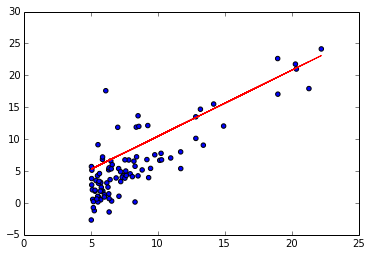
\includegraphics[max size={\textwidth}{\textheight}]{Trabalho 1_files/Trabalho 1_14_0.png}
    \par
    \end{center}
    
            \end{InvisibleVerbatim}
            
        
    
\subsubsection{Plot do gráfico de EQM por época}

    % Make sure that atleast 4 lines are below the HR
    \needspace{4\baselineskip}

    
        \vspace{6pt}
        \makebox[0.1\linewidth]{\smaller\hfill\tt\color{nbframe-in-prompt}In\hspace{4pt}{[}180{]}:\hspace{4pt}}\\*
        \vspace{-2.65\baselineskip}
        \begin{ColorVerbatim}
            \vspace{-0.7\baselineskip}
            \begin{Verbatim}[commandchars=\\\{\}]
\PY{n}{plot2d}\PY{p}{(}\PY{n+nb}{xrange}\PY{p}{(}\PY{n+nb}{len}\PY{p}{(}\PY{n}{eqms}\PY{p}{)}\PY{p}{)}\PY{p}{,} \PY{n}{eqms}\PY{p}{)}
\end{Verbatim}

            
                \vspace{-0.2\baselineskip}
            
        \end{ColorVerbatim}
    

    

        % If the first block is an image, minipage the image.  Else
        % request a certain amount of space for the input text.
        \needspace{4\baselineskip}
        
        

            % Add document contents.
            
                \begin{InvisibleVerbatim}
                \vspace{-0.5\baselineskip}
    \begin{center}
    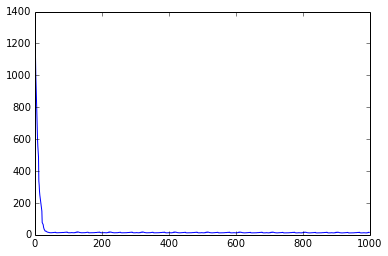
\includegraphics[max size={\textwidth}{\textheight}]{Trabalho 1_files/Trabalho 1_16_0.png}
    \par
    \end{center}
    
            \end{InvisibleVerbatim}
            
        
    
\subsubsection{Valor final dos coeficientes}

    % Make sure that atleast 4 lines are below the HR
    \needspace{4\baselineskip}

    
        \vspace{6pt}
        \makebox[0.1\linewidth]{\smaller\hfill\tt\color{nbframe-in-prompt}In\hspace{4pt}{[}181{]}:\hspace{4pt}}\\*
        \vspace{-2.65\baselineskip}
        \begin{ColorVerbatim}
            \vspace{-0.7\baselineskip}
            \begin{Verbatim}[commandchars=\\\{\}]
\PY{k}{print} \PY{n}{ws}
\end{Verbatim}

            
                \vspace{-0.2\baselineskip}
            
        \end{ColorVerbatim}
    

    

        % If the first block is an image, minipage the image.  Else
        % request a certain amount of space for the input text.
        \needspace{4\baselineskip}
        
        

            % Add document contents.
            
                \begin{InvisibleVerbatim}
                \vspace{-0.5\baselineskip}
\begin{alltt}[0.083977384040390332, 1.0367198512504761]
\end{alltt}

            \end{InvisibleVerbatim}
            
        
    
\subsubsection{Comentários: Através do gráfico ``épocas x EQM'' é possível verificar
que o algoritmo está ``aprendendo'' ? Comente.}
Considerando que uma diminuição dos erros do modelo em predições sobre
dados do training-set representam aprendizado, pode-se sim afirmar que
o  algoritmo está "aprendendo".
Podemos pensar cada época de treinamento como um incremento no
aprendizado.
\subsubsection{Exemplo de utilização da função, para um conjunto de dados
simples(função 2*x)}

    % Make sure that atleast 4 lines are below the HR
    \needspace{4\baselineskip}

    
        \vspace{6pt}
        \makebox[0.1\linewidth]{\smaller\hfill\tt\color{nbframe-in-prompt}In\hspace{4pt}{[}182{]}:\hspace{4pt}}\\*
        \vspace{-2.65\baselineskip}
        \begin{ColorVerbatim}
            \vspace{-0.7\baselineskip}
            \begin{Verbatim}[commandchars=\\\{\}]
\PY{n}{ws}\PY{p}{,} \PY{n}{eqms} \PY{o}{=} \PY{n}{grad\PYZus{}desc\PYZus{}estoq}\PY{p}{(}\PY{p}{[}\PY{p}{[}\PY{n}{x}\PY{p}{]} \PY{k}{for} \PY{n}{x} \PY{o+ow}{in} \PY{n+nb}{xrange}\PY{p}{(}\PY{l+m+mi}{40}\PY{p}{)}\PY{p}{]}\PY{p}{,} \PY{p}{[}\PY{l+m+mi}{2}\PY{o}{*}\PY{n}{x} \PY{k}{for} \PY{n}{x} \PY{o+ow}{in} \PY{n+nb}{xrange}\PY{p}{(}\PY{l+m+mi}{40}\PY{p}{)}\PY{p}{]}\PY{p}{,} \PY{n}{alfa}\PY{o}{=}\PY{l+m+mf}{0.001}\PY{p}{,} \PY{n}{epocas}\PY{o}{=}\PY{l+m+mi}{1000}\PY{p}{,} \PY{n}{plot}\PY{o}{=}\PY{n+nb+bp}{True}\PY{p}{)}
\end{Verbatim}

            
                \vspace{-0.2\baselineskip}
            
        \end{ColorVerbatim}
    

    

        % If the first block is an image, minipage the image.  Else
        % request a certain amount of space for the input text.
        \needspace{4\baselineskip}
        
        

            % Add document contents.
            
                \begin{InvisibleVerbatim}
                \vspace{-0.5\baselineskip}
    \begin{center}
    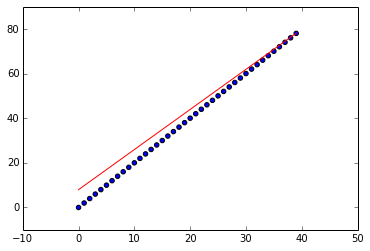
\includegraphics[max size={\textwidth}{\textheight}]{Trabalho 1_files/Trabalho 1_22_0.png}
    \par
    \end{center}
    
            \end{InvisibleVerbatim}
            
        
    


    % Make sure that atleast 4 lines are below the HR
    \needspace{4\baselineskip}

    
        \vspace{6pt}
        \makebox[0.1\linewidth]{\smaller\hfill\tt\color{nbframe-in-prompt}In\hspace{4pt}{[}183{]}:\hspace{4pt}}\\*
        \vspace{-2.65\baselineskip}
        \begin{ColorVerbatim}
            \vspace{-0.7\baselineskip}
            \begin{Verbatim}[commandchars=\\\{\}]
\PY{n}{plot2d}\PY{p}{(}\PY{n+nb}{xrange}\PY{p}{(}\PY{n+nb}{len}\PY{p}{(}\PY{n}{eqms}\PY{p}{)}\PY{p}{)}\PY{p}{,} \PY{n}{eqms}\PY{p}{)}
\end{Verbatim}

            
                \vspace{-0.2\baselineskip}
            
        \end{ColorVerbatim}
    

    

        % If the first block is an image, minipage the image.  Else
        % request a certain amount of space for the input text.
        \needspace{4\baselineskip}
        
        

            % Add document contents.
            
                \begin{InvisibleVerbatim}
                \vspace{-0.5\baselineskip}
    \begin{center}
    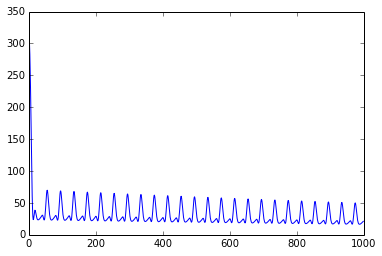
\includegraphics[max size={\textwidth}{\textheight}]{Trabalho 1_files/Trabalho 1_23_0.png}
    \par
    \end{center}
    
            \end{InvisibleVerbatim}
            
        
    
\subsubsection{Utilizando o modelo do scikit-learn}

    % Make sure that atleast 4 lines are below the HR
    \needspace{4\baselineskip}

    
        \vspace{6pt}
        \makebox[0.1\linewidth]{\smaller\hfill\tt\color{nbframe-in-prompt}In\hspace{4pt}{[}184{]}:\hspace{4pt}}\\*
        \vspace{-2.65\baselineskip}
        \begin{ColorVerbatim}
            \vspace{-0.7\baselineskip}
            \begin{Verbatim}[commandchars=\\\{\}]
\PY{k+kn}{from} \PY{n+nn}{sklearn} \PY{k+kn}{import} \PY{n}{linear\PYZus{}model}
\PY{n}{clf} \PY{o}{=} \PY{n}{linear\PYZus{}model}\PY{o}{.}\PY{n}{LinearRegression}\PY{p}{(}\PY{p}{)}
\PY{n}{clf}\PY{o}{.}\PY{n}{fit}\PY{p}{(}\PY{p}{[}\PY{p}{[}\PY{n}{x}\PY{p}{]} \PY{k}{for} \PY{n}{x} \PY{o+ow}{in} \PY{n+nb}{xrange}\PY{p}{(}\PY{l+m+mi}{20}\PY{p}{)}\PY{p}{]}\PY{p}{,} \PY{p}{[}\PY{n}{x}\PY{o}{*}\PY{l+m+mi}{2} \PY{o}{+} \PY{l+m+mi}{4} \PY{k}{for} \PY{n}{x} \PY{o+ow}{in} \PY{n+nb}{xrange}\PY{p}{(}\PY{l+m+mi}{20}\PY{p}{)}\PY{p}{]}\PY{p}{)}

\PY{k}{print} \PY{n}{clf}\PY{o}{.}\PY{n}{coef\PYZus{}}
\end{Verbatim}

            
                \vspace{-0.2\baselineskip}
            
        \end{ColorVerbatim}
    

    

        % If the first block is an image, minipage the image.  Else
        % request a certain amount of space for the input text.
        \needspace{4\baselineskip}
        
        

            % Add document contents.
            
                \begin{InvisibleVerbatim}
                \vspace{-0.5\baselineskip}
\begin{alltt}[ 2.]
\end{alltt}

            \end{InvisibleVerbatim}
            
        
    
\part{Questão 2}

    % Make sure that atleast 4 lines are below the HR
    \needspace{4\baselineskip}

    
        \vspace{6pt}
        \makebox[0.1\linewidth]{\smaller\hfill\tt\color{nbframe-in-prompt}In\hspace{4pt}{[}185{]}:\hspace{4pt}}\\*
        \vspace{-2.65\baselineskip}
        \begin{ColorVerbatim}
            \vspace{-0.7\baselineskip}
            \begin{Verbatim}[commandchars=\\\{\}]
\PY{n}{X}\PY{p}{,} \PY{n}{Y} \PY{o}{=} \PY{n}{carregar}\PY{p}{(}\PY{n}{FILENAMES}\PY{p}{[}\PY{l+m+mi}{1}\PY{p}{]}\PY{p}{)}
\end{Verbatim}

            
                \vspace{-0.2\baselineskip}
            
        \end{ColorVerbatim}
    
\subsubsection{Gráfico do Y pela feature 1}

    % Make sure that atleast 4 lines are below the HR
    \needspace{4\baselineskip}

    
        \vspace{6pt}
        \makebox[0.1\linewidth]{\smaller\hfill\tt\color{nbframe-in-prompt}In\hspace{4pt}{[}186{]}:\hspace{4pt}}\\*
        \vspace{-2.65\baselineskip}
        \begin{ColorVerbatim}
            \vspace{-0.7\baselineskip}
            \begin{Verbatim}[commandchars=\\\{\}]
\PY{n}{scatter2d}\PY{p}{(}\PY{n}{X}\PY{p}{[}\PY{p}{:}\PY{p}{,} \PY{l+m+mi}{0}\PY{p}{]}\PY{p}{,} \PY{n}{Y}\PY{p}{)}
\end{Verbatim}

            
                \vspace{-0.2\baselineskip}
            
        \end{ColorVerbatim}
    

    

        % If the first block is an image, minipage the image.  Else
        % request a certain amount of space for the input text.
        \needspace{4\baselineskip}
        
        

            % Add document contents.
            
                \begin{InvisibleVerbatim}
                \vspace{-0.5\baselineskip}
    \begin{center}
    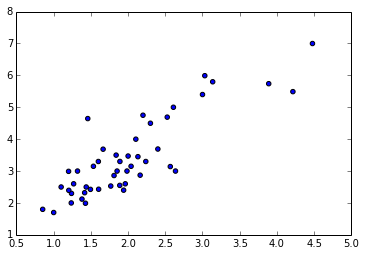
\includegraphics[max size={\textwidth}{\textheight}]{Trabalho 1_files/Trabalho 1_29_0.png}
    \par
    \end{center}
    
            \end{InvisibleVerbatim}
            
        
    
\subsubsection{Gráfico do Y pela feature 2}

    % Make sure that atleast 4 lines are below the HR
    \needspace{4\baselineskip}

    
        \vspace{6pt}
        \makebox[0.1\linewidth]{\smaller\hfill\tt\color{nbframe-in-prompt}In\hspace{4pt}{[}187{]}:\hspace{4pt}}\\*
        \vspace{-2.65\baselineskip}
        \begin{ColorVerbatim}
            \vspace{-0.7\baselineskip}
            \begin{Verbatim}[commandchars=\\\{\}]
\PY{n}{scatter2d}\PY{p}{(}\PY{n}{X}\PY{p}{[}\PY{p}{:}\PY{p}{,} \PY{l+m+mi}{1}\PY{p}{]}\PY{p}{,} \PY{n}{Y}\PY{p}{)}
\end{Verbatim}

            
                \vspace{-0.2\baselineskip}
            
        \end{ColorVerbatim}
    

    

        % If the first block is an image, minipage the image.  Else
        % request a certain amount of space for the input text.
        \needspace{4\baselineskip}
        
        

            % Add document contents.
            
                \begin{InvisibleVerbatim}
                \vspace{-0.5\baselineskip}
    \begin{center}
    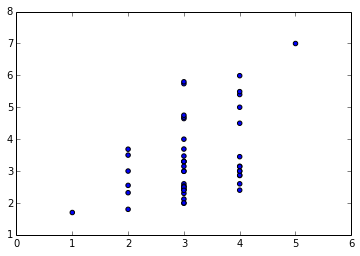
\includegraphics[max size={\textwidth}{\textheight}]{Trabalho 1_files/Trabalho 1_31_0.png}
    \par
    \end{center}
    
            \end{InvisibleVerbatim}
            
        
    
\subsubsection{Execução do gradiente descendente estocástico}

    % Make sure that atleast 4 lines are below the HR
    \needspace{4\baselineskip}

    
        \vspace{6pt}
        \makebox[0.1\linewidth]{\smaller\hfill\tt\color{nbframe-in-prompt}In\hspace{4pt}{[}188{]}:\hspace{4pt}}\\*
        \vspace{-2.65\baselineskip}
        \begin{ColorVerbatim}
            \vspace{-0.7\baselineskip}
            \begin{Verbatim}[commandchars=\\\{\}]
\PY{n}{ws}\PY{p}{,} \PY{n}{eqms} \PY{o}{=} \PY{n}{grad\PYZus{}desc\PYZus{}estoq}\PY{p}{(}\PY{n}{X}\PY{p}{,} \PY{n}{Y}\PY{p}{,} \PY{n}{alfa}\PY{o}{=}\PY{l+m+mf}{0.01}\PY{p}{,} \PY{n}{epocas}\PY{o}{=}\PY{l+m+mi}{100}\PY{p}{)}
\end{Verbatim}

            
                \vspace{-0.2\baselineskip}
            
        \end{ColorVerbatim}
    
\subsubsection{Plot do gráfico de EQM por época}

    % Make sure that atleast 4 lines are below the HR
    \needspace{4\baselineskip}

    
        \vspace{6pt}
        \makebox[0.1\linewidth]{\smaller\hfill\tt\color{nbframe-in-prompt}In\hspace{4pt}{[}189{]}:\hspace{4pt}}\\*
        \vspace{-2.65\baselineskip}
        \begin{ColorVerbatim}
            \vspace{-0.7\baselineskip}
            \begin{Verbatim}[commandchars=\\\{\}]
\PY{n}{plot2d}\PY{p}{(}\PY{n+nb}{xrange}\PY{p}{(}\PY{n+nb}{len}\PY{p}{(}\PY{n}{eqms}\PY{p}{)}\PY{p}{)}\PY{p}{,} \PY{n}{eqms}\PY{p}{)}
\end{Verbatim}

            
                \vspace{-0.2\baselineskip}
            
        \end{ColorVerbatim}
    

    

        % If the first block is an image, minipage the image.  Else
        % request a certain amount of space for the input text.
        \needspace{4\baselineskip}
        
        

            % Add document contents.
            
                \begin{InvisibleVerbatim}
                \vspace{-0.5\baselineskip}
    \begin{center}
    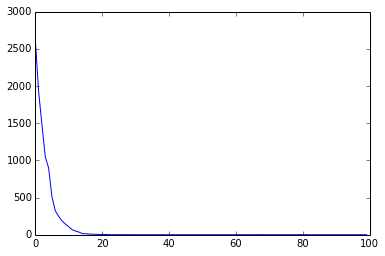
\includegraphics[max size={\textwidth}{\textheight}]{Trabalho 1_files/Trabalho 1_35_0.png}
    \par
    \end{center}
    
            \end{InvisibleVerbatim}
            
        
    
\subsubsection{Coeficientes}

    % Make sure that atleast 4 lines are below the HR
    \needspace{4\baselineskip}

    
        \vspace{6pt}
        \makebox[0.1\linewidth]{\smaller\hfill\tt\color{nbframe-in-prompt}In\hspace{4pt}{[}190{]}:\hspace{4pt}}\\*
        \vspace{-2.65\baselineskip}
        \begin{ColorVerbatim}
            \vspace{-0.7\baselineskip}
            \begin{Verbatim}[commandchars=\\\{\}]
\PY{k}{print} \PY{n}{ws}
\end{Verbatim}

            
                \vspace{-0.2\baselineskip}
            
        \end{ColorVerbatim}
    

    

        % If the first block is an image, minipage the image.  Else
        % request a certain amount of space for the input text.
        \needspace{4\baselineskip}
        
        

            % Add document contents.
            
                \begin{InvisibleVerbatim}
                \vspace{-0.5\baselineskip}
\begin{alltt}[4.8428259014688733, 1.2367045451514695, -1.144013877275414]
\end{alltt}

            \end{InvisibleVerbatim}
            
        
    
\subsubsection{Comentários: Através do gráfico ``épocas x EQM'' é possível verificar
que o algoritmo está ``aprendendo'' ? Comente.}
Mesma resposta para a mesma pergunta da questão 1.
\subsubsection{Regressão com o método dos mínimos quadrados}

    % Make sure that atleast 4 lines are below the HR
    \needspace{4\baselineskip}

    
        \vspace{6pt}
        \makebox[0.1\linewidth]{\smaller\hfill\tt\color{nbframe-in-prompt}In\hspace{4pt}{[}191{]}:\hspace{4pt}}\\*
        \vspace{-2.65\baselineskip}
        \begin{ColorVerbatim}
            \vspace{-0.7\baselineskip}
            \begin{Verbatim}[commandchars=\\\{\}]
\PY{k}{def} \PY{n+nf}{add\PYZus{}ones\PYZus{}left}\PY{p}{(}\PY{n}{X}\PY{p}{)}\PY{p}{:}
    \PY{n}{X\PYZus{}com\PYZus{}1s} \PY{o}{=} \PY{n}{np}\PY{o}{.}\PY{n}{ones}\PY{p}{(}\PY{p}{(}\PY{n}{X}\PY{o}{.}\PY{n}{shape}\PY{p}{[}\PY{l+m+mi}{0}\PY{p}{]}\PY{p}{,} \PY{n}{X}\PY{o}{.}\PY{n}{shape}\PY{p}{[}\PY{l+m+mi}{1}\PY{p}{]}\PY{o}{+}\PY{l+m+mi}{1}\PY{p}{)}\PY{p}{)}
    \PY{n}{X\PYZus{}com\PYZus{}1s}\PY{p}{[}\PY{p}{:}\PY{p}{,} \PY{l+m+mi}{1}\PY{p}{:}\PY{p}{]} \PY{o}{=} \PY{n}{X}
    
    \PY{k}{return} \PY{n}{X\PYZus{}com\PYZus{}1s}
    
\PY{k}{def} \PY{n+nf}{lsm}\PY{p}{(}\PY{n}{X}\PY{p}{,} \PY{n}{Y}\PY{p}{)}\PY{p}{:}
    \PY{k+kn}{import} \PY{n+nn}{numpy} \PY{k+kn}{as} \PY{n+nn}{np}
    
    \PY{c}{\PYZsh{} 1s da coluna do peso w0}
    \PY{n}{X\PYZus{}com\PYZus{}1s} \PY{o}{=} \PY{n}{add\PYZus{}ones\PYZus{}left}\PY{p}{(}\PY{n}{X}\PY{p}{)}
    
    \PY{n}{Xt} \PY{o}{=} \PY{n}{np}\PY{o}{.}\PY{n}{transpose}\PY{p}{(}\PY{n}{X\PYZus{}com\PYZus{}1s}\PY{p}{)}
    \PY{n}{Xt\PYZus{}dot\PYZus{}X} \PY{o}{=} \PY{n}{np}\PY{o}{.}\PY{n}{dot}\PY{p}{(}\PY{n}{Xt}\PY{p}{,} \PY{n}{X\PYZus{}com\PYZus{}1s}\PY{p}{)}
    \PY{n}{Xt\PYZus{}dot\PYZus{}X\PYZus{}inv} \PY{o}{=} \PY{n}{np}\PY{o}{.}\PY{n}{linalg}\PY{o}{.}\PY{n}{solve}\PY{p}{(}\PY{n}{Xt\PYZus{}dot\PYZus{}X}\PY{p}{,} \PY{n}{np}\PY{o}{.}\PY{n}{identity}\PY{p}{(}\PY{n+nb}{len}\PY{p}{(}\PY{n}{Xt\PYZus{}dot\PYZus{}X}\PY{p}{)}\PY{p}{)}\PY{p}{)}
    \PY{n}{Xt\PYZus{}dot\PYZus{}X\PYZus{}inv\PYZus{}Xt} \PY{o}{=} \PY{n}{np}\PY{o}{.}\PY{n}{dot}\PY{p}{(}\PY{n}{Xt\PYZus{}dot\PYZus{}X\PYZus{}inv}\PY{p}{,} \PY{n}{Xt}\PY{p}{)}
    \PY{k}{return} \PY{n}{np}\PY{o}{.}\PY{n}{dot}\PY{p}{(}\PY{n}{Xt\PYZus{}dot\PYZus{}X\PYZus{}inv\PYZus{}Xt}\PY{p}{,} \PY{n}{Y}\PY{p}{)}
\end{Verbatim}

            
                \vspace{-0.2\baselineskip}
            
        \end{ColorVerbatim}
    
\subsubsection{\begin{itemize}
\itemsep1pt\parskip0pt\parsep0pt
\item
  Encontre os coeficientes da regressão utilizando o método dos mínimos
  quadrados.
\end{itemize}}

    % Make sure that atleast 4 lines are below the HR
    \needspace{4\baselineskip}

    
        \vspace{6pt}
        \makebox[0.1\linewidth]{\smaller\hfill\tt\color{nbframe-in-prompt}In\hspace{4pt}{[}192{]}:\hspace{4pt}}\\*
        \vspace{-2.65\baselineskip}
        \begin{ColorVerbatim}
            \vspace{-0.7\baselineskip}
            \begin{Verbatim}[commandchars=\\\{\}]
\PY{n}{lsm}\PY{p}{(}\PY{n}{X}\PY{p}{,} \PY{n}{Y}\PY{p}{)}
\end{Verbatim}

            
                \vspace{-0.2\baselineskip}
            
        \end{ColorVerbatim}
    

    

        % If the first block is an image, minipage the image.  Else
        % request a certain amount of space for the input text.
        \needspace{4\baselineskip}
        
        

            % Add document contents.
            
                \makebox[0.1\linewidth]{\smaller\hfill\tt\color{nbframe-out-prompt}Out\hspace{4pt}{[}192{]}:\hspace{4pt}}\\*
                \vspace{-2.55\baselineskip}\begin{InvisibleVerbatim}
                \vspace{-0.5\baselineskip}
\begin{alltt}array([ 0.8959791 ,  1.39210674, -0.08738019])\end{alltt}

            \end{InvisibleVerbatim}
            
        
    
\subsubsection{Utilizando o modelo do scikit-learn}

    % Make sure that atleast 4 lines are below the HR
    \needspace{4\baselineskip}

    
        \vspace{6pt}
        \makebox[0.1\linewidth]{\smaller\hfill\tt\color{nbframe-in-prompt}In\hspace{4pt}{[}193{]}:\hspace{4pt}}\\*
        \vspace{-2.65\baselineskip}
        \begin{ColorVerbatim}
            \vspace{-0.7\baselineskip}
            \begin{Verbatim}[commandchars=\\\{\}]
\PY{k+kn}{from} \PY{n+nn}{sklearn} \PY{k+kn}{import} \PY{n}{linear\PYZus{}model}
\PY{n}{clf} \PY{o}{=} \PY{n}{linear\PYZus{}model}\PY{o}{.}\PY{n}{LinearRegression}\PY{p}{(}\PY{p}{)}
\PY{n}{clf}\PY{o}{.}\PY{n}{fit}\PY{p}{(}\PY{n}{add\PYZus{}ones\PYZus{}left}\PY{p}{(}\PY{n}{X}\PY{p}{)}\PY{p}{,} \PY{n}{Y}\PY{p}{)}

\PY{k}{print} \PY{n}{clf}\PY{o}{.}\PY{n}{coef\PYZus{}}
\end{Verbatim}

            
                \vspace{-0.2\baselineskip}
            
        \end{ColorVerbatim}
    

    

        % If the first block is an image, minipage the image.  Else
        % request a certain amount of space for the input text.
        \needspace{4\baselineskip}
        
        

            % Add document contents.
            
                \begin{InvisibleVerbatim}
                \vspace{-0.5\baselineskip}
\begin{alltt}[ 0.          1.39210674 -0.08738019]
\end{alltt}

            \end{InvisibleVerbatim}
            
        
    
\subsubsection{Comentários: Os valores obtidos pelos dois métodos são iguais? Comente.}
Não. O segundo método oferece um resultado mais preciso que o
primeiro, mas tem um custo computacional maior.
\part{Questão 3}

    % Make sure that atleast 4 lines are below the HR
    \needspace{4\baselineskip}

    
        \vspace{6pt}
        \makebox[0.1\linewidth]{\smaller\hfill\tt\color{nbframe-in-prompt}In\hspace{4pt}{[}194{]}:\hspace{4pt}}\\*
        \vspace{-2.65\baselineskip}
        \begin{ColorVerbatim}
            \vspace{-0.7\baselineskip}
            \begin{Verbatim}[commandchars=\\\{\}]
\PY{n}{X}\PY{p}{,} \PY{n}{Y} \PY{o}{=} \PY{n}{carregar}\PY{p}{(}\PY{n}{FILENAMES}\PY{p}{[}\PY{l+m+mi}{2}\PY{p}{]}\PY{p}{)}
\end{Verbatim}

            
                \vspace{-0.2\baselineskip}
            
        \end{ColorVerbatim}
    
\subsubsection{Divisão dos dados em training-set e test-set}

    % Make sure that atleast 4 lines are below the HR
    \needspace{4\baselineskip}

    
        \vspace{6pt}
        \makebox[0.1\linewidth]{\smaller\hfill\tt\color{nbframe-in-prompt}In\hspace{4pt}{[}195{]}:\hspace{4pt}}\\*
        \vspace{-2.65\baselineskip}
        \begin{ColorVerbatim}
            \vspace{-0.7\baselineskip}
            \begin{Verbatim}[commandchars=\\\{\}]
\PY{n}{X\PYZus{}training} \PY{o}{=} \PY{n}{X}\PY{p}{[}\PY{p}{:}\PY{l+m+mi}{30}\PY{p}{]}
\PY{n}{Y\PYZus{}training} \PY{o}{=} \PY{n}{Y}\PY{p}{[}\PY{p}{:}\PY{l+m+mi}{30}\PY{p}{]}

\PY{n}{X\PYZus{}test} \PY{o}{=} \PY{n}{X}\PY{p}{[}\PY{l+m+mi}{30}\PY{p}{:}\PY{p}{]}
\PY{n}{Y\PYZus{}test} \PY{o}{=} \PY{n}{Y}\PY{p}{[}\PY{l+m+mi}{30}\PY{p}{:}\PY{p}{]}
\end{Verbatim}

            
                \vspace{-0.2\baselineskip}
            
        \end{ColorVerbatim}
    
\subsubsection{\begin{itemize}
\itemsep1pt\parskip0pt\parsep0pt
\item
  Encontre os coeficientes da regressão utilizando o método dos mínimos
  quadrados regularizado para os seguintes valores de λ = {[}0 1 2 3 4
  5{]}. Utilize o conjunto de treinamento.
\end{itemize}}

    % Make sure that atleast 4 lines are below the HR
    \needspace{4\baselineskip}

    
        \vspace{6pt}
        \makebox[0.1\linewidth]{\smaller\hfill\tt\color{nbframe-in-prompt}In\hspace{4pt}{[}196{]}:\hspace{4pt}}\\*
        \vspace{-2.65\baselineskip}
        \begin{ColorVerbatim}
            \vspace{-0.7\baselineskip}
            \begin{Verbatim}[commandchars=\\\{\}]
\PY{k}{def} \PY{n+nf}{lsm\PYZus{}regularizado}\PY{p}{(}\PY{n}{X}\PY{p}{,} \PY{n}{Y}\PY{p}{,} \PY{n}{lamb}\PY{o}{=}\PY{l+m+mi}{0}\PY{p}{)}\PY{p}{:}
    \PY{k+kn}{import} \PY{n+nn}{numpy} \PY{k+kn}{as} \PY{n+nn}{np}
    
    \PY{c}{\PYZsh{} 1s da coluna do peso w0}
    \PY{n}{X\PYZus{}com\PYZus{}1s} \PY{o}{=} \PY{n}{add\PYZus{}ones\PYZus{}left}\PY{p}{(}\PY{n}{X}\PY{p}{)}
    
    \PY{n}{Xt} \PY{o}{=} \PY{n}{np}\PY{o}{.}\PY{n}{transpose}\PY{p}{(}\PY{n}{X\PYZus{}com\PYZus{}1s}\PY{p}{)}
    \PY{n}{Xt\PYZus{}dot\PYZus{}X} \PY{o}{=} \PY{n}{np}\PY{o}{.}\PY{n}{dot}\PY{p}{(}\PY{n}{Xt}\PY{p}{,} \PY{n}{X\PYZus{}com\PYZus{}1s}\PY{p}{)}
    \PY{n}{Xt\PYZus{}dot\PYZus{}X\PYZus{}plus\PYZus{}lamb} \PY{o}{=} \PY{n}{Xt\PYZus{}dot\PYZus{}X} \PY{o}{+} \PY{n}{np}\PY{o}{.}\PY{n}{identity}\PY{p}{(}\PY{n}{Xt\PYZus{}dot\PYZus{}X}\PY{o}{.}\PY{n}{shape}\PY{p}{[}\PY{l+m+mi}{0}\PY{p}{]}\PY{p}{)}\PY{o}{*}\PY{n}{lamb}
    \PY{n}{Xt\PYZus{}dot\PYZus{}X\PYZus{}inv} \PY{o}{=} \PY{n}{np}\PY{o}{.}\PY{n}{linalg}\PY{o}{.}\PY{n}{solve}\PY{p}{(}\PY{n}{Xt\PYZus{}dot\PYZus{}X\PYZus{}plus\PYZus{}lamb}\PY{p}{,} \PY{n}{np}\PY{o}{.}\PY{n}{identity}\PY{p}{(}\PY{n+nb}{len}\PY{p}{(}\PY{n}{Xt\PYZus{}dot\PYZus{}X\PYZus{}plus\PYZus{}lamb}\PY{p}{)}\PY{p}{)}\PY{p}{)}
    \PY{n}{Xt\PYZus{}dot\PYZus{}X\PYZus{}inv\PYZus{}Xt} \PY{o}{=} \PY{n}{np}\PY{o}{.}\PY{n}{dot}\PY{p}{(}\PY{n}{Xt\PYZus{}dot\PYZus{}X\PYZus{}inv}\PY{p}{,} \PY{n}{Xt}\PY{p}{)}
    \PY{k}{return} \PY{n}{np}\PY{o}{.}\PY{n}{dot}\PY{p}{(}\PY{n}{Xt\PYZus{}dot\PYZus{}X\PYZus{}inv\PYZus{}Xt}\PY{p}{,} \PY{n}{Y}\PY{p}{)}
\end{Verbatim}

            
                \vspace{-0.2\baselineskip}
            
        \end{ColorVerbatim}
    


    % Make sure that atleast 4 lines are below the HR
    \needspace{4\baselineskip}

    
        \vspace{6pt}
        \makebox[0.1\linewidth]{\smaller\hfill\tt\color{nbframe-in-prompt}In\hspace{4pt}{[}197{]}:\hspace{4pt}}\\*
        \vspace{-2.65\baselineskip}
        \begin{ColorVerbatim}
            \vspace{-0.7\baselineskip}
            \begin{Verbatim}[commandchars=\\\{\}]
\PY{n}{coeficientes} \PY{o}{=} \PY{p}{[}\PY{p}{]}
\PY{n}{lambdas} \PY{o}{=} \PY{p}{[}\PY{l+m+mi}{0}\PY{p}{,}\PY{l+m+mi}{1}\PY{p}{,}\PY{l+m+mi}{2}\PY{p}{,}\PY{l+m+mi}{3}\PY{p}{,}\PY{l+m+mi}{4}\PY{p}{,}\PY{l+m+mi}{5}\PY{p}{]}

\PY{k}{for} \PY{n}{lamb} \PY{o+ow}{in} \PY{n}{lambdas}\PY{p}{:}
    \PY{n}{coeficientes}\PY{o}{.}\PY{n}{append}\PY{p}{(}\PY{p}{[}\PY{n}{lamb}\PY{p}{,} \PY{n}{lsm\PYZus{}regularizado}\PY{p}{(}\PY{n}{X\PYZus{}training}\PY{p}{,} \PY{n}{Y\PYZus{}training}\PY{p}{,} \PY{n}{lamb}\PY{o}{=}\PY{n}{lamb}\PY{p}{)}\PY{p}{]}\PY{p}{)}
\end{Verbatim}

            
                \vspace{-0.2\baselineskip}
            
        \end{ColorVerbatim}
    


    % Make sure that atleast 4 lines are below the HR
    \needspace{4\baselineskip}

    
        \vspace{6pt}
        \makebox[0.1\linewidth]{\smaller\hfill\tt\color{nbframe-in-prompt}In\hspace{4pt}{[}198{]}:\hspace{4pt}}\\*
        \vspace{-2.65\baselineskip}
        \begin{ColorVerbatim}
            \vspace{-0.7\baselineskip}
            \begin{Verbatim}[commandchars=\\\{\}]
\PY{n}{coefs\PYZus{}frame} \PY{o}{=} \PY{p}{[}\PY{p}{]}
\PY{k+kn}{from} \PY{n+nn}{pandas} \PY{k+kn}{import} \PY{n}{DataFrame}

\PY{n}{coefs} \PY{o}{=} \PY{n}{np}\PY{o}{.}\PY{n}{array}\PY{p}{(}\PY{p}{[}\PY{n}{coef} \PY{k}{for} \PY{p}{[}\PY{n}{\PYZus{}}\PY{p}{,} \PY{n}{coef}\PY{p}{]} \PY{o+ow}{in} \PY{n}{coeficientes}\PY{p}{]}\PY{p}{)}

\PY{n}{as\PYZus{}dict} \PY{o}{=} \PY{p}{\PYZob{}}\PY{l+s}{\PYZdq{}}\PY{l+s}{w0}\PY{l+s}{\PYZdq{}}\PY{p}{:}\PY{n}{coefs}\PY{p}{[}\PY{p}{:}\PY{p}{,}\PY{l+m+mi}{0}\PY{p}{]}\PY{p}{,} \PY{l+s}{\PYZdq{}}\PY{l+s}{w1}\PY{l+s}{\PYZdq{}}\PY{p}{:}\PY{n}{coefs}\PY{p}{[}\PY{p}{:}\PY{p}{,}\PY{l+m+mi}{1}\PY{p}{]}\PY{p}{,} \PY{l+s}{\PYZdq{}}\PY{l+s}{w2}\PY{l+s}{\PYZdq{}}\PY{p}{:}\PY{n}{coefs}\PY{p}{[}\PY{p}{:}\PY{p}{,}\PY{l+m+mi}{2}\PY{p}{]}\PY{p}{,} \PY{l+s}{\PYZdq{}}\PY{l+s}{w3}\PY{l+s}{\PYZdq{}}\PY{p}{:}\PY{n}{coefs}\PY{p}{[}\PY{p}{:}\PY{p}{,}\PY{l+m+mi}{3}\PY{p}{]}\PY{p}{,} \PY{l+s}{\PYZdq{}}\PY{l+s}{w4}\PY{l+s}{\PYZdq{}}\PY{p}{:}\PY{n}{coefs}\PY{p}{[}\PY{p}{:}\PY{p}{,}\PY{l+m+mi}{4}\PY{p}{]}\PY{p}{,} \PY{l+s}{\PYZdq{}}\PY{l+s}{w5}\PY{l+s}{\PYZdq{}}\PY{p}{:}\PY{n}{coefs}\PY{p}{[}\PY{p}{:}\PY{p}{,}\PY{l+m+mi}{5}\PY{p}{]}\PY{p}{\PYZcb{}}

\PY{n}{coefs\PYZus{}frame} \PY{o}{=} \PY{n}{DataFrame}\PY{p}{(}\PY{n}{data}\PY{o}{=}\PY{n}{as\PYZus{}dict}\PY{p}{)}

\PY{n}{coefs\PYZus{}frame}
\end{Verbatim}

            
                \vspace{-0.2\baselineskip}
            
        \end{ColorVerbatim}
    

    

        % If the first block is an image, minipage the image.  Else
        % request a certain amount of space for the input text.
        \needspace{4\baselineskip}
        
        

            % Add document contents.
            
                \makebox[0.1\linewidth]{\smaller\hfill\tt\color{nbframe-out-prompt}Out\hspace{4pt}{[}198{]}:\hspace{4pt}}\\*
                \vspace{-2.55\baselineskip}\begin{InvisibleVerbatim}
                \vspace{-0.5\baselineskip}
\begin{alltt}         w0        w1        w2        w3        w4        w5
0  0.792989  2.056501  0.121439 -1.161379  0.062729 -0.391102
1  0.111568  1.327679  0.254142  0.220779  0.049086 -0.254957
2  0.097677  1.154551  0.274012  0.287010  0.058775 -0.123092
3  0.098098  1.043871  0.291524  0.298925  0.070535 -0.038295
4  0.100460  0.963394  0.307166  0.298476  0.081888  0.019792
5  0.103095  0.901191  0.320989  0.294309  0.092194  0.061640\end{alltt}

            \end{InvisibleVerbatim}
            
        
    
\subsubsection{Comentários: Quais variáveis parecem ser menos relevantes para a
regressão?}
Para cada lambda, ordenamos crescentemente as variáveis, em valores
absolutos, ficando com:


    % Make sure that atleast 4 lines are below the HR
    \needspace{4\baselineskip}

    
        \vspace{6pt}
        \makebox[0.1\linewidth]{\smaller\hfill\tt\color{nbframe-in-prompt}In\hspace{4pt}{[}199{]}:\hspace{4pt}}\\*
        \vspace{-2.65\baselineskip}
        \begin{ColorVerbatim}
            \vspace{-0.7\baselineskip}
            \begin{Verbatim}[commandchars=\\\{\}]
\PY{n}{coefs\PYZus{}frame} \PY{o}{=} \PY{p}{[}\PY{p}{]}
\PY{k+kn}{from} \PY{n+nn}{pandas} \PY{k+kn}{import} \PY{n}{DataFrame}

\PY{n}{coefs} \PY{o}{=} \PY{n}{np}\PY{o}{.}\PY{n}{abs}\PY{p}{(}\PY{n}{np}\PY{o}{.}\PY{n}{array}\PY{p}{(}\PY{p}{[}\PY{n}{coef} \PY{k}{for} \PY{p}{[}\PY{n}{\PYZus{}}\PY{p}{,} \PY{n}{coef}\PY{p}{]} \PY{o+ow}{in} \PY{n}{coeficientes}\PY{p}{]}\PY{p}{)}\PY{p}{)}

\PY{n}{as\PYZus{}dicts} \PY{o}{=} \PY{p}{[}\PY{p}{\PYZob{}}\PY{l+s}{\PYZdq{}}\PY{l+s}{lambda 0}\PY{l+s}{\PYZdq{}}\PY{p}{:}\PY{n}{coefs}\PY{p}{[}\PY{l+m+mi}{0}\PY{p}{,}\PY{p}{:}\PY{p}{]}\PY{p}{\PYZcb{}}\PY{p}{,} \PY{p}{\PYZob{}}\PY{l+s}{\PYZdq{}}\PY{l+s}{lambda 1}\PY{l+s}{\PYZdq{}}\PY{p}{:}\PY{n}{coefs}\PY{p}{[}\PY{l+m+mi}{1}\PY{p}{,}\PY{p}{:}\PY{p}{]}\PY{p}{\PYZcb{}}\PY{p}{,} \PY{p}{\PYZob{}}\PY{l+s}{\PYZdq{}}\PY{l+s}{lambda 2}\PY{l+s}{\PYZdq{}}\PY{p}{:}\PY{n}{coefs}\PY{p}{[}\PY{l+m+mi}{2}\PY{p}{,}\PY{p}{:}\PY{p}{]}\PY{p}{\PYZcb{}}\PY{p}{,} \PY{p}{\PYZob{}}\PY{l+s}{\PYZdq{}}\PY{l+s}{lambda 3}\PY{l+s}{\PYZdq{}}\PY{p}{:}\PY{n}{coefs}\PY{p}{[}\PY{l+m+mi}{3}\PY{p}{,}\PY{p}{:}\PY{p}{]}\PY{p}{\PYZcb{}}\PY{p}{,} \PY{p}{\PYZob{}}\PY{l+s}{\PYZdq{}}\PY{l+s}{lambda 4}\PY{l+s}{\PYZdq{}}\PY{p}{:}\PY{n}{coefs}\PY{p}{[}\PY{l+m+mi}{4}\PY{p}{,}\PY{p}{:}\PY{p}{]}\PY{p}{\PYZcb{}}\PY{p}{,} \PY{p}{\PYZob{}}\PY{l+s}{\PYZdq{}}\PY{l+s}{lambda 5}\PY{l+s}{\PYZdq{}}\PY{p}{:}\PY{n}{coefs}\PY{p}{[}\PY{l+m+mi}{5}\PY{p}{,}\PY{p}{:}\PY{p}{]}\PY{p}{\PYZcb{}}\PY{p}{]}

\PY{n}{coefs\PYZus{}frames} \PY{o}{=} \PY{p}{[}\PY{n}{DataFrame}\PY{p}{(}\PY{n}{data}\PY{o}{=}\PY{n}{as\PYZus{}dict}\PY{p}{)} \PY{k}{for} \PY{n}{as\PYZus{}dict} \PY{o+ow}{in} \PY{n}{as\PYZus{}dicts}\PY{p}{]}

\PY{k}{for} \PY{n}{i} \PY{o+ow}{in} \PY{n+nb}{xrange}\PY{p}{(}\PY{l+m+mi}{6}\PY{p}{)}\PY{p}{:}
    \PY{k}{print} \PY{n}{coefs\PYZus{}frames}\PY{p}{[}\PY{n}{i}\PY{p}{]}\PY{o}{.}\PY{n}{sort}\PY{p}{(}\PY{l+s}{\PYZdq{}}\PY{l+s}{lambda }\PY{l+s+si}{\PYZpc{}s}\PY{l+s}{\PYZdq{}} \PY{o}{\PYZpc{}} \PY{n+nb}{str}\PY{p}{(}\PY{n}{i}\PY{p}{)}\PY{p}{)}
\end{Verbatim}

            
                \vspace{-0.2\baselineskip}
            
        \end{ColorVerbatim}
    

    

        % If the first block is an image, minipage the image.  Else
        % request a certain amount of space for the input text.
        \needspace{4\baselineskip}
        
        

            % Add document contents.
            
                \begin{InvisibleVerbatim}
                \vspace{-0.5\baselineskip}
\begin{alltt}   lambda 0
4  0.062729
2  0.121439
5  0.391102
0  0.792989
3  1.161379
1  2.056501
   lambda 1
4  0.049086
0  0.111568
3  0.220779
2  0.254142
5  0.254957
1  1.327679
   lambda 2
4  0.058775
0  0.097677
5  0.123092
2  0.274012
3  0.287010
1  1.154551
   lambda 3
5  0.038295
4  0.070535
0  0.098098
2  0.291524
3  0.298925
1  1.043871
   lambda 4
5  0.019792
4  0.081888
0  0.100460
3  0.298476
2  0.307166
1  0.963394
   lambda 5
5  0.061640
4  0.092194
0  0.103095
3  0.294309
2  0.320989
1  0.901191
\end{alltt}

            \end{InvisibleVerbatim}
            
        
    

Para lambdas em {0, 1, 2} o w4 foi a variável com menor valor
absoluto.
Já para lambdas em {3, 4, 5} o w5 foi a variável com menor valor
absoluto.
\subsubsection{\begin{itemize}
\itemsep1pt\parskip0pt\parsep0pt
\item
  Encontrar o valor do EQM para os dados de treinamento e de teste para
  cada um dos valores de λ.
\end{itemize}}

    % Make sure that atleast 4 lines are below the HR
    \needspace{4\baselineskip}

    
        \vspace{6pt}
        \makebox[0.1\linewidth]{\smaller\hfill\tt\color{nbframe-in-prompt}In\hspace{4pt}{[}200{]}:\hspace{4pt}}\\*
        \vspace{-2.65\baselineskip}
        \begin{ColorVerbatim}
            \vspace{-0.7\baselineskip}
            \begin{Verbatim}[commandchars=\\\{\}]
\PY{n}{eqms\PYZus{}por\PYZus{}lambda} \PY{o}{=} \PY{p}{[}\PY{p}{]}

\PY{k}{for} \PY{n}{lamb}\PY{p}{,} \PY{n}{coefs} \PY{o+ow}{in} \PY{n}{coeficientes}\PY{p}{:}
    \PY{n}{pred\PYZus{}training} \PY{o}{=} \PY{p}{[}\PY{n}{eq\PYZus{}1grau}\PY{p}{(}\PY{n}{coefs}\PY{p}{,} \PY{n}{xs}\PY{p}{)} \PY{k}{for} \PY{n}{xs} \PY{o+ow}{in} \PY{n}{X\PYZus{}training}\PY{p}{]}
    \PY{n}{eqm\PYZus{}training}\PY{o}{=} \PY{n}{eqm}\PY{p}{(}\PY{n}{pred\PYZus{}training}\PY{p}{,} \PY{n}{Y\PYZus{}training}\PY{p}{)}
    
    \PY{n}{pred\PYZus{}test} \PY{o}{=} \PY{p}{[}\PY{n}{eq\PYZus{}1grau}\PY{p}{(}\PY{n}{coefs}\PY{p}{,} \PY{n}{xs}\PY{p}{)} \PY{k}{for} \PY{n}{xs} \PY{o+ow}{in} \PY{n}{X\PYZus{}test}\PY{p}{]}
    \PY{n}{eqm\PYZus{}test} \PY{o}{=} \PY{n}{eqm}\PY{p}{(}\PY{n}{pred\PYZus{}test}\PY{p}{,} \PY{n}{Y\PYZus{}test}\PY{p}{)}
    
    \PY{n}{eqms\PYZus{}por\PYZus{}lambda}\PY{o}{.}\PY{n}{append}\PY{p}{(}\PY{p}{[}\PY{n}{eqm\PYZus{}training}\PY{p}{,} \PY{n}{eqm\PYZus{}test}\PY{p}{]}\PY{p}{)}
    
\PY{n}{eqms\PYZus{}por\PYZus{}lambda} \PY{o}{=} \PY{n}{np}\PY{o}{.}\PY{n}{array}\PY{p}{(}\PY{n}{eqms\PYZus{}por\PYZus{}lambda}\PY{p}{)}
\end{Verbatim}

            
                \vspace{-0.2\baselineskip}
            
        \end{ColorVerbatim}
    
\subsubsection{Gráfico de EQM x training-set}

    % Make sure that atleast 4 lines are below the HR
    \needspace{4\baselineskip}

    
        \vspace{6pt}
        \makebox[0.1\linewidth]{\smaller\hfill\tt\color{nbframe-in-prompt}In\hspace{4pt}{[}201{]}:\hspace{4pt}}\\*
        \vspace{-2.65\baselineskip}
        \begin{ColorVerbatim}
            \vspace{-0.7\baselineskip}
            \begin{Verbatim}[commandchars=\\\{\}]
\PY{n}{plot2d}\PY{p}{(}\PY{n+nb}{xrange}\PY{p}{(}\PY{l+m+mi}{6}\PY{p}{)}\PY{p}{,} \PY{n}{eqms\PYZus{}por\PYZus{}lambda}\PY{p}{[}\PY{p}{:}\PY{p}{,}\PY{l+m+mi}{0}\PY{p}{]}\PY{p}{)}
\end{Verbatim}

            
                \vspace{-0.2\baselineskip}
            
        \end{ColorVerbatim}
    

    

        % If the first block is an image, minipage the image.  Else
        % request a certain amount of space for the input text.
        \needspace{4\baselineskip}
        
        

            % Add document contents.
            
                \begin{InvisibleVerbatim}
                \vspace{-0.5\baselineskip}
    \begin{center}
    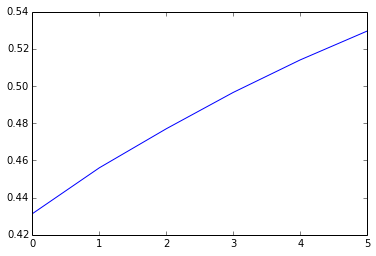
\includegraphics[max size={\textwidth}{\textheight}]{Trabalho 1_files/Trabalho 1_63_0.png}
    \par
    \end{center}
    
            \end{InvisibleVerbatim}
            
        
    
\subsubsection{Gráfico de EQM x test-set}

    % Make sure that atleast 4 lines are below the HR
    \needspace{4\baselineskip}

    
        \vspace{6pt}
        \makebox[0.1\linewidth]{\smaller\hfill\tt\color{nbframe-in-prompt}In\hspace{4pt}{[}202{]}:\hspace{4pt}}\\*
        \vspace{-2.65\baselineskip}
        \begin{ColorVerbatim}
            \vspace{-0.7\baselineskip}
            \begin{Verbatim}[commandchars=\\\{\}]
\PY{n}{plot2d}\PY{p}{(}\PY{n+nb}{xrange}\PY{p}{(}\PY{l+m+mi}{6}\PY{p}{)}\PY{p}{,} \PY{n}{eqms\PYZus{}por\PYZus{}lambda}\PY{p}{[}\PY{p}{:}\PY{p}{,}\PY{l+m+mi}{1}\PY{p}{]}\PY{p}{)}
\end{Verbatim}

            
                \vspace{-0.2\baselineskip}
            
        \end{ColorVerbatim}
    

    

        % If the first block is an image, minipage the image.  Else
        % request a certain amount of space for the input text.
        \needspace{4\baselineskip}
        
        

            % Add document contents.
            
                \begin{InvisibleVerbatim}
                \vspace{-0.5\baselineskip}
    \begin{center}
    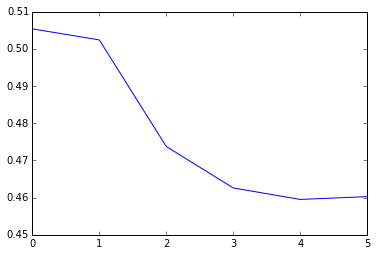
\includegraphics[max size={\textwidth}{\textheight}]{Trabalho 1_files/Trabalho 1_65_0.png}
    \par
    \end{center}
    
            \end{InvisibleVerbatim}
            
        
    
\subsubsection{Comentários: Como os valores dos coeficientes variam com λ ? Explique o
motivo.}

    % Make sure that atleast 4 lines are below the HR
    \needspace{4\baselineskip}

    
        \vspace{6pt}
        \makebox[0.1\linewidth]{\smaller\hfill\tt\color{nbframe-in-prompt}In\hspace{4pt}{[}203{]}:\hspace{4pt}}\\*
        \vspace{-2.65\baselineskip}
        \begin{ColorVerbatim}
            \vspace{-0.7\baselineskip}
            \begin{Verbatim}[commandchars=\\\{\}]
\PY{k}{for} \PY{n}{lamb}\PY{p}{,} \PY{n}{coefs} \PY{o+ow}{in} \PY{n}{coeficientes}\PY{p}{:}
    \PY{k}{print} \PY{l+s}{\PYZdq{}}\PY{l+s}{Lambda:}\PY{l+s}{\PYZdq{}}\PY{p}{,} \PY{n}{lamb}\PY{p}{,} \PY{l+s}{\PYZdq{}}\PY{l+s}{Média dos coeficientes:}\PY{l+s}{\PYZdq{}}\PY{p}{,} \PY{n+nb}{sum}\PY{p}{(}\PY{n}{np}\PY{o}{.}\PY{n}{abs}\PY{p}{(}\PY{n}{coefs}\PY{p}{)}\PY{p}{)}\PY{o}{/}\PY{n+nb}{len}\PY{p}{(}\PY{n}{coefs}\PY{p}{)}
\end{Verbatim}

            
                \vspace{-0.2\baselineskip}
            
        \end{ColorVerbatim}
    

    

        % If the first block is an image, minipage the image.  Else
        % request a certain amount of space for the input text.
        \needspace{4\baselineskip}
        
        

            % Add document contents.
            
                \begin{InvisibleVerbatim}
                \vspace{-0.5\baselineskip}
\begin{alltt}Lambda: 0 Média dos coeficientes: 0.764356552684
Lambda: 1 Média dos coeficientes: 0.369701833015
Lambda: 2 Média dos coeficientes: 0.332519429917
Lambda: 3 Média dos coeficientes: 0.306874650909
Lambda: 4 Média dos coeficientes: 0.2951959092
Lambda: 5 Média dos coeficientes: 0.2955695343
\end{alltt}

            \end{InvisibleVerbatim}
            
        
    

Como se pode observar pelos dados acima, quanto maior o lambda, menor
é a média absoluta dos coeficientes.
O motivo é o fato de ter sido utilizada uma técnica de
regularização(suavização) que diminui o valor dos coeficientes
proporcionalmente às suas influências nos resultados.
\subsubsection{Comente o crescimento/decrescimento dos erros presente nas figuras EQM x
λ}
Pode-se perceber que quanto maior o lambda da regularização, maior
torna-se o EQM para os dados de treinamento e menor torna-se o EQM
para os dados de teste.
Uma das possíveis causas para tal situação é que há dados no training-
set que causam uma grande variação no modelo, variação esta que não
reflete a função que representa os dados. Tal problema é denominado
overfitting e, para resolvê-lo, utilizam-se técnicas de regularização
de forma a diminuir tais distorções.

        

        \renewcommand{\indexname}{Index}
        \printindex

    % End of document
    \end{document}


